\documentclass{mimosis}

\usepackage{metalogo}
\usepackage{graphicx} % allow embedded images
  \setkeys{Gin}{width=\linewidth,totalheight=\textheight,keepaspectratio}
  \graphicspath{{../figs/}} % set of paths to search for images
\usepackage{amsmath}  % extended mathematics
\usepackage{units}

%%%%%%%%%%%%%%%%%%%%%%%%%%%%%%%%%%%%%%%%%%%%%%%%%%%%%%%%%%%%%%%%%%%%%%%%
% Some of my favourite personal adjustments
%%%%%%%%%%%%%%%%%%%%%%%%%%%%%%%%%%%%%%%%%%%%%%%%%%%%%%%%%%%%%%%%%%%%%%%%
%
% These are the adjustments that I consider necessary for typesetting
% a nice thesis. However, they are *not* included in the template, as
% I do not want to force you to use them.

% This ensures that I am able to typeset bold font in table while still aligning the numbers
% correctly.
\usepackage{etoolbox}

\usepackage[binary-units=true]{siunitx}
\DeclareSIUnit\px{px}

\sisetup{%
  detect-all           = true,
  detect-family        = true,
  detect-mode          = true,
  detect-shape         = true,
  detect-weight        = true,
  detect-inline-weight = math,
}

%%%%%%%%%%%%%%%%%%%%%%%%%%%%%%%%%%%%%%%%%%%%%%%%%%%%%%%%%%%%%%%%%%%%%%%%
% Hyperlinks & bookmarks
%%%%%%%%%%%%%%%%%%%%%%%%%%%%%%%%%%%%%%%%%%%%%%%%%%%%%%%%%%%%%%%%%%%%%%%%

\usepackage[%
  colorlinks = true,
  citecolor  = RoyalBlue,
  linkcolor  = RoyalBlue,
  urlcolor   = RoyalBlue,
  unicode,
  ]{hyperref}

\usepackage{bookmark}

%%%%%%%%%%%%%%%%%%%%%%%%%%%%%%%%%%%%%%%%%%%%%%%%%%%%%%%%%%%%%%%%%%%%%%%%
% Bibliography
%%%%%%%%%%%%%%%%%%%%%%%%%%%%%%%%%%%%%%%%%%%%%%%%%%%%%%%%%%%%%%%%%%%%%%%%
%
% I like the bibliography to be extremely plain, showing only a numeric
% identifier and citing everything in simple brackets. The first names,
% if present, will be initialized. DOIs and URLs will be preserved.

\usepackage[%
  autocite     = plain,
  backend      = bibtex,
  doi          = true,
  url          = true,
  giveninits   = true,
  hyperref     = true,
  maxbibnames  = 99,
  maxcitenames = 99,
  sortcites    = true,
  style        = numeric,
  ]{biblatex}

%%%%%%%%%%%%%%%%%%%%%%%%%%%%%%%%%%%%%%%%%%%%%%%%%%%%%%%%%%%%%%%%%%%%%%%%
% Some adjustments to make the bibliography more clean
%%%%%%%%%%%%%%%%%%%%%%%%%%%%%%%%%%%%%%%%%%%%%%%%%%%%%%%%%%%%%%%%%%%%%%%%
%
% The subsequent commands do the following:
%  - Removing the month field from the bibliography
%  - Fixing the Oxford commma
%  - Suppress the "in" for journal articles
%  - Remove the parentheses of the year in an article
%  - Delimit volume and issue of an article by a colon ":" instead of
%    a dot ""
%  - Use commas to separate the location of publishers from their name
%  - Remove the abbreviation for technical reports
%  - Display the label of bibliographic entries without brackets in the
%    bibliography
%  - Ensure that DOIs are followed by a non-breakable space
%  - Use hair spaces between initials of authors
%  - Make the font size of citations smaller
%  - Fixing ordinal numbers (1st, 2nd, 3rd, and so) on by using
%    superscripts

% Remove the month field from the bibliography. It does not serve a good
% purpose, I guess. And often, it cannot be used because the journals
% have some crazy issue policies.
\AtEveryBibitem{\clearfield{month}}
\AtEveryCitekey{\clearfield{month}}

% Fixing the Oxford comma. Not sure whether this is the proper solution.
% More information is available under [1] and [2].
%
% [1] http://tex.stackexchange.com/questions/97712/biblatex-apa-style-is-missing-a-comma-in-the-references-why
% [2] http://tex.stackexchange.com/questions/44048/use-et-al-in-biblatex-custom-style
%
\AtBeginBibliography{%
  \renewcommand*{\finalnamedelim}{%
    \ifthenelse{\value{listcount} > 2}{%
      \addcomma
      \addspace
      \bibstring{and}%
    }{%
      \addspace
      \bibstring{and}%
    }
  }
}

% Suppress "in" for journal articles. This is unnecessary in my opinion
% because the journal title is typeset in italics anyway.
\renewbibmacro{in:}{%
  \ifentrytype{article}
  {%
  }%
  % else
  {%
    \printtext{\bibstring{in}\intitlepunct}%
  }%
}

% Remove the parentheses for the year in an article. This removes a lot
% of undesired parentheses in the bibliography, thereby improving the
% readability. Moreover, it makes the look of the bibliography more
% consistent.
\renewbibmacro*{issue+date}{%
  \setunit{\addcomma\space}
    \iffieldundef{issue}
      {\usebibmacro{date}}
      {\printfield{issue}%
       \setunit*{\addspace}%
       \usebibmacro{date}}%
  \newunit}

% Delimit the volume and the number of an article by a colon instead of
% by a dot, which I consider to be more readable.
\renewbibmacro*{volume+number+eid}{%
  \printfield{volume}%
  \setunit*{\addcolon}%
  \printfield{number}%
  \setunit{\addcomma\space}%
  \printfield{eid}%
}

% Do not use a colon for the publisher location. Instead, connect
% publisher, location, and date via commas.
\renewbibmacro*{publisher+location+date}{%
  \printlist{publisher}%
  \setunit*{\addcomma\space}%
  \printlist{location}%
  \setunit*{\addcomma\space}%
  \usebibmacro{date}%
  \newunit%
}

% Ditto for other entry types.
\renewbibmacro*{organization+location+date}{%
  \printlist{location}%
  \setunit*{\addcomma\space}%
  \printlist{organization}%
  \setunit*{\addcomma\space}%
  \usebibmacro{date}%
  \newunit%
}

% Display the label of a bibliographic entry in bare style, without any
% brackets. I like this more than the default.
%
% Note that this is *really* the proper and official way of doing this.
\DeclareFieldFormat{labelnumberwidth}{#1\adddot}

% Ensure that DOIs are followed by a non-breakable space.
\DeclareFieldFormat{doi}{%
  \mkbibacro{DOI}\addcolon\addnbspace
    \ifhyperref
      {\href{http://dx.doi.org/#1}{\nolinkurl{#1}}}
      %
      {\nolinkurl{#1}}
}

% Use proper hair spaces between initials as suggested by Bringhurst and
% others.
\renewcommand*\bibinitdelim {\addnbthinspace}
\renewcommand*\bibnamedelima{\addnbthinspace}
\renewcommand*\bibnamedelimb{\addnbthinspace}
\renewcommand*\bibnamedelimi{\addnbthinspace}

% Make the font size of citations smaller. Depending on your selected
% font, you might not need this.
\renewcommand*{\citesetup}{%
  \biburlsetup
  \small
}

\DeclareLanguageMapping{english}{english-mimosis}

\addbibresource{References.bib}

%%%%%%%%%%%%%%%%%%%%%%%%%%%%%%%%%%%%%%%%%%%%%%%%%%%%%%%%%%%%%%%%%%%%%%%%
% Fonts
%%%%%%%%%%%%%%%%%%%%%%%%%%%%%%%%%%%%%%%%%%%%%%%%%%%%%%%%%%%%%%%%%%%%%%%%

\ifxetexorluatex
  \setmainfont{Minion Pro}
\else
  \usepackage[lf]{ebgaramond}
  \usepackage[oldstyle,scale=0.7]{sourcecodepro}
  \singlespacing
\fi

\renewcommand{\th}{\textsuperscript{\textup{th}}\xspace}

\newacronym[description={Principal component analysis}]{PCA}{PCA}{principal component analysis}
\newacronym                                            {SNF}{SNF}{Smith normal form}
\newacronym[description={Topological data analysis}]   {TDA}{TDA}{topological data analysis}

\newglossaryentry{LaTeX}{%
  name        = {\LaTeX},
  description = {A document preparation system},
  sort        = {LaTeX},
}

\newglossaryentry{Real numbers}{%
  name        = {$\real$},
  description = {The set of real numbers},
  sort        = {Real numbers},
}

\makeindex
\makeglossaries

%%%%%%%%%%%%%%%%%%%%%%%%%%%%%%%%%%%%%%%%%%%%%%%%%%%%%%%%%%%%%%%%%%%%%%%%
% Incipit
%%%%%%%%%%%%%%%%%%%%%%%%%%%%%%%%%%%%%%%%%%%%%%%%%%%%%%%%%%%%%%%%%%%%%%%%

\title{\texttt{latex-mimosis}}
\subtitle{A minimal, modern \LaTeX{} package for typesetting your thesis}
\author{Bastian Rieck}

\begin{document}

\frontmatter
%  \include{Sources/Title}
%  \include{Sources/Abstract}

  \tableofcontents

\mainmatter
  \chapter{Introduction}
  The field of reinforcement learning (RL) has long relied on heuristics, sampling and hand written feature recognition. To learn end to end, directly from high level input, has been a significant challenge. Utilizing (convolutional) neural networks the field of deep learning has succeeded to recognize features from high level input. Here we take a look at Deep Q networks (DQN) a successful approach to end-to-end reinforcement learning. The Q-table from classic Q-learning is replaced by a neural network where the training of the network mimics the Q-learning update formula.

There are a number of significant challenges. Reinforcement learning generates its own data, measures must be taken to prevent feedback loops. In deep learning the network immediately gets feedback weather it was correct or not. In Reinforcement Learning there might be hundreds of not thousands of steps between an action and the reward. An RL agent must be able to deal with delayed rewards. 

Here we implement a DQN agent to solve the tasks mountain car and breakout. Mountain car is a simple control based task where one challenge is that the reward is only given after the task is completed. Breakout is one of the classic Atari 2600 games successfully learned in the famous "Human-level control through deep reinforcement learning"\cite{DQN} paper. I will use this to adapt the implementation for mountain car to work on breakout. I will use two of the learning techniques introduced there: experience replay and infrequent weight updates. For the mountain car problem we will experiment with agents with various memory sizes for experience replay and with and without infrequent weight updates. The breakout problem requires carefully tuning, together with lots of training, which did not leave time to experiment.

In the next section I discuss the theory of DQN, the challenges introduced above and how these are partially solved with experience replay and infrequent weight updates. Then I will discuss my implementation of DQN for mountain car. This is followed by a section on the performance while experimenting with the agent. Next I shift the focus to breakout, detailing how the implementation for mountain car needed to be adjusted to get the breakout agent to learn. After this we take an in depth look at the training of the agent and how it performed. And in the final section of this report we conclude weather our agents have succeeded and how they could be improved. In the appendix at the end we detail how our agents can be tested.
  \chapter{Theory}
  Here we will give a short theoretical introduction to deep Q-networks (DQN). A DQN is capable of learning a diverse array of challanging tasks without hand coded domain specific knowledge. Recieving only the state of its envirement it returns one of the given possible actions, it then gets feedback in the form of a reward.

DQN is based on Q-learning or action-value learning. In Q-learning the Q function \autoref{eq:Q} calculates the quality of a state-action combination. The outcome is then stored in the Q table and can be used to create more Q values. When an action is required the action with the highest Q value in the table is performed.

\begin{align} \label{eq:Q}
Q^{n e w}\left(s_{t}, a_{t}\right) \leftarrow 
(1-\alpha)\cdot\underbrace{Q\left(s_{t}, a_{t}\right)}_{\text {old value }} 
%
+\underbrace{\alpha}_{\text {learning rate }} \cdot (\underbrace{r_{t}}_{\text {reward }}
+\underbrace{\gamma}_{\text {discount factor }} \cdot \underbrace{\max _{a} Q\left(s_{t+1}, a\right)}_{\text {estimate of future value }})
\end{align}

Here $Q^{new}$ is the new Q-value for the state $s_t$ and action $a_t$. We calculate it by combining the old Q value with new information we learned as we transitioned to state $s_{t+1}$ by action $a_t$. We weigh the combination with the learning rate $\alpha$, the higher the learning rate the higher the impact of the new information. The new information consists of the reward $r_t$ and Q value of the best action we can take from here\footnote{as the best action is the action with the highest Q value we can add the maximum Q value corrosponding to the new state $s_{t+1}$ we are now in.}: $\max _{a} Q\left(s_{t+1}, a\right)$ We additionally weigh this by the discount factor $\gamma$ which determines how importend future rewards are. 

Initially the Q table is empty and it will need training. The only way to fill the table is to performce random actions, using the reward to find the Q-value. A good strategy is to let the rate of random actions $\epsilon$ decrease throughout the training process. Starting at $\epsilon = 1$ and ending at $\epsilon = 0.1$.

This table based way of learning has only limited applications. For example if we where to apply Q-learning to the mountain car problem \autoref{sec:mountain_car} we would immidiately run into a problem. The needed Q-table would need to be infinite\footnote{ignoring the limited resolution of the \texttt{doubles} used to represent the state of the car}. While this can be solved by discretizing the input before the Q-learning algorithm there are many more complex problem where this is not feasable. One of these is our second problem, the atari game breakout, see \autoref{sec:breakout}. For this we turn to DQN.

In DQN the optimal action-value is approximated by a neural network. When we need to perform an action we ask the neural network to make predictions for the Q-values for all the different possible actions. We then pick the action with the highest predicted Q-value. 
 
Initially the neural network will behave like the empty table from Q-learning, not knowing the right Q value. However as we train the network it wil converge to the Q value. The network is trained with as input the state and action and as label the correct Q-value as calculated from \autoref{eq:Q}, getting $Q\left(s_{t+1}, a\right)$ and $Q\left(s_{t}, a\right)$ by asking the network to make a prediction for input $[s_{t+1}, a]$ and $[s_{t}, a]$ respectively. 

There is a danger in using a neural network. The reinforcement learning can become unstable\cite{triad}. This is attributed to the \textit{deadly triad}: function approximation, bootstrapping and off policy learning. The Q-function is approximated by the neural network based on features recognized in states states that should have a different Q-values may share the same features leading to loops in behavior. Bootstrapping, or basing the new Q-values partially on the old may exaggerate the problems introduced by the imperfect approximation. Finally DQN uses off policy learning it converges less well then on policy learning.

Mnih, Koray Kavukcuoglu, and Silver\cite{DQN} adress these instabilities using a replay buffer. By storing the states, actions and corrosponding reward the network can learn on results out of order. This breaks feedback loops solving the unstability described above. Another significant improvement made is infrequent weight updates. Here a seperate network is used for the predictions. This prevents the network from returning values based on newly learned behaviour while training causing those behaviours to be reinforced entering a feedback loop. Once in a while the network used for prediction is replaced with the current training network.
  \chapter{Mountain Car}
  \label{sec:breakout}
Here the agent needs to master the atari game breakout, see \autoref{fig:breakout}. The agent controls a small bar at the bottem of the screen with possible actions: move left, move right or stay. A ball moves with constant speed through the envirement. If the agent positions the small bar such that the ball hits the bar the ball inverts its vertical velocity bouncing upwards. Whenever the ball hits the bottem of the screen it disappears, the agent loses a life (it starts with 5) and a new ball is introduced with a random direction downwards. When the ball hits the left and right side of the screen the horizontal velocity is inverted making it bounce of the walls. Somewhat below the top of the screen is a stack of rows of blocks. Whenever the ball hits one of the blocks: the block disappears, the ball inverts its vertical velocity and the agent is rewarded with score one for the current timestep. If the ball hits the top of the screen its vertical velocity is inverted, bouncing it off the top. 

\begin{marginfigure}
    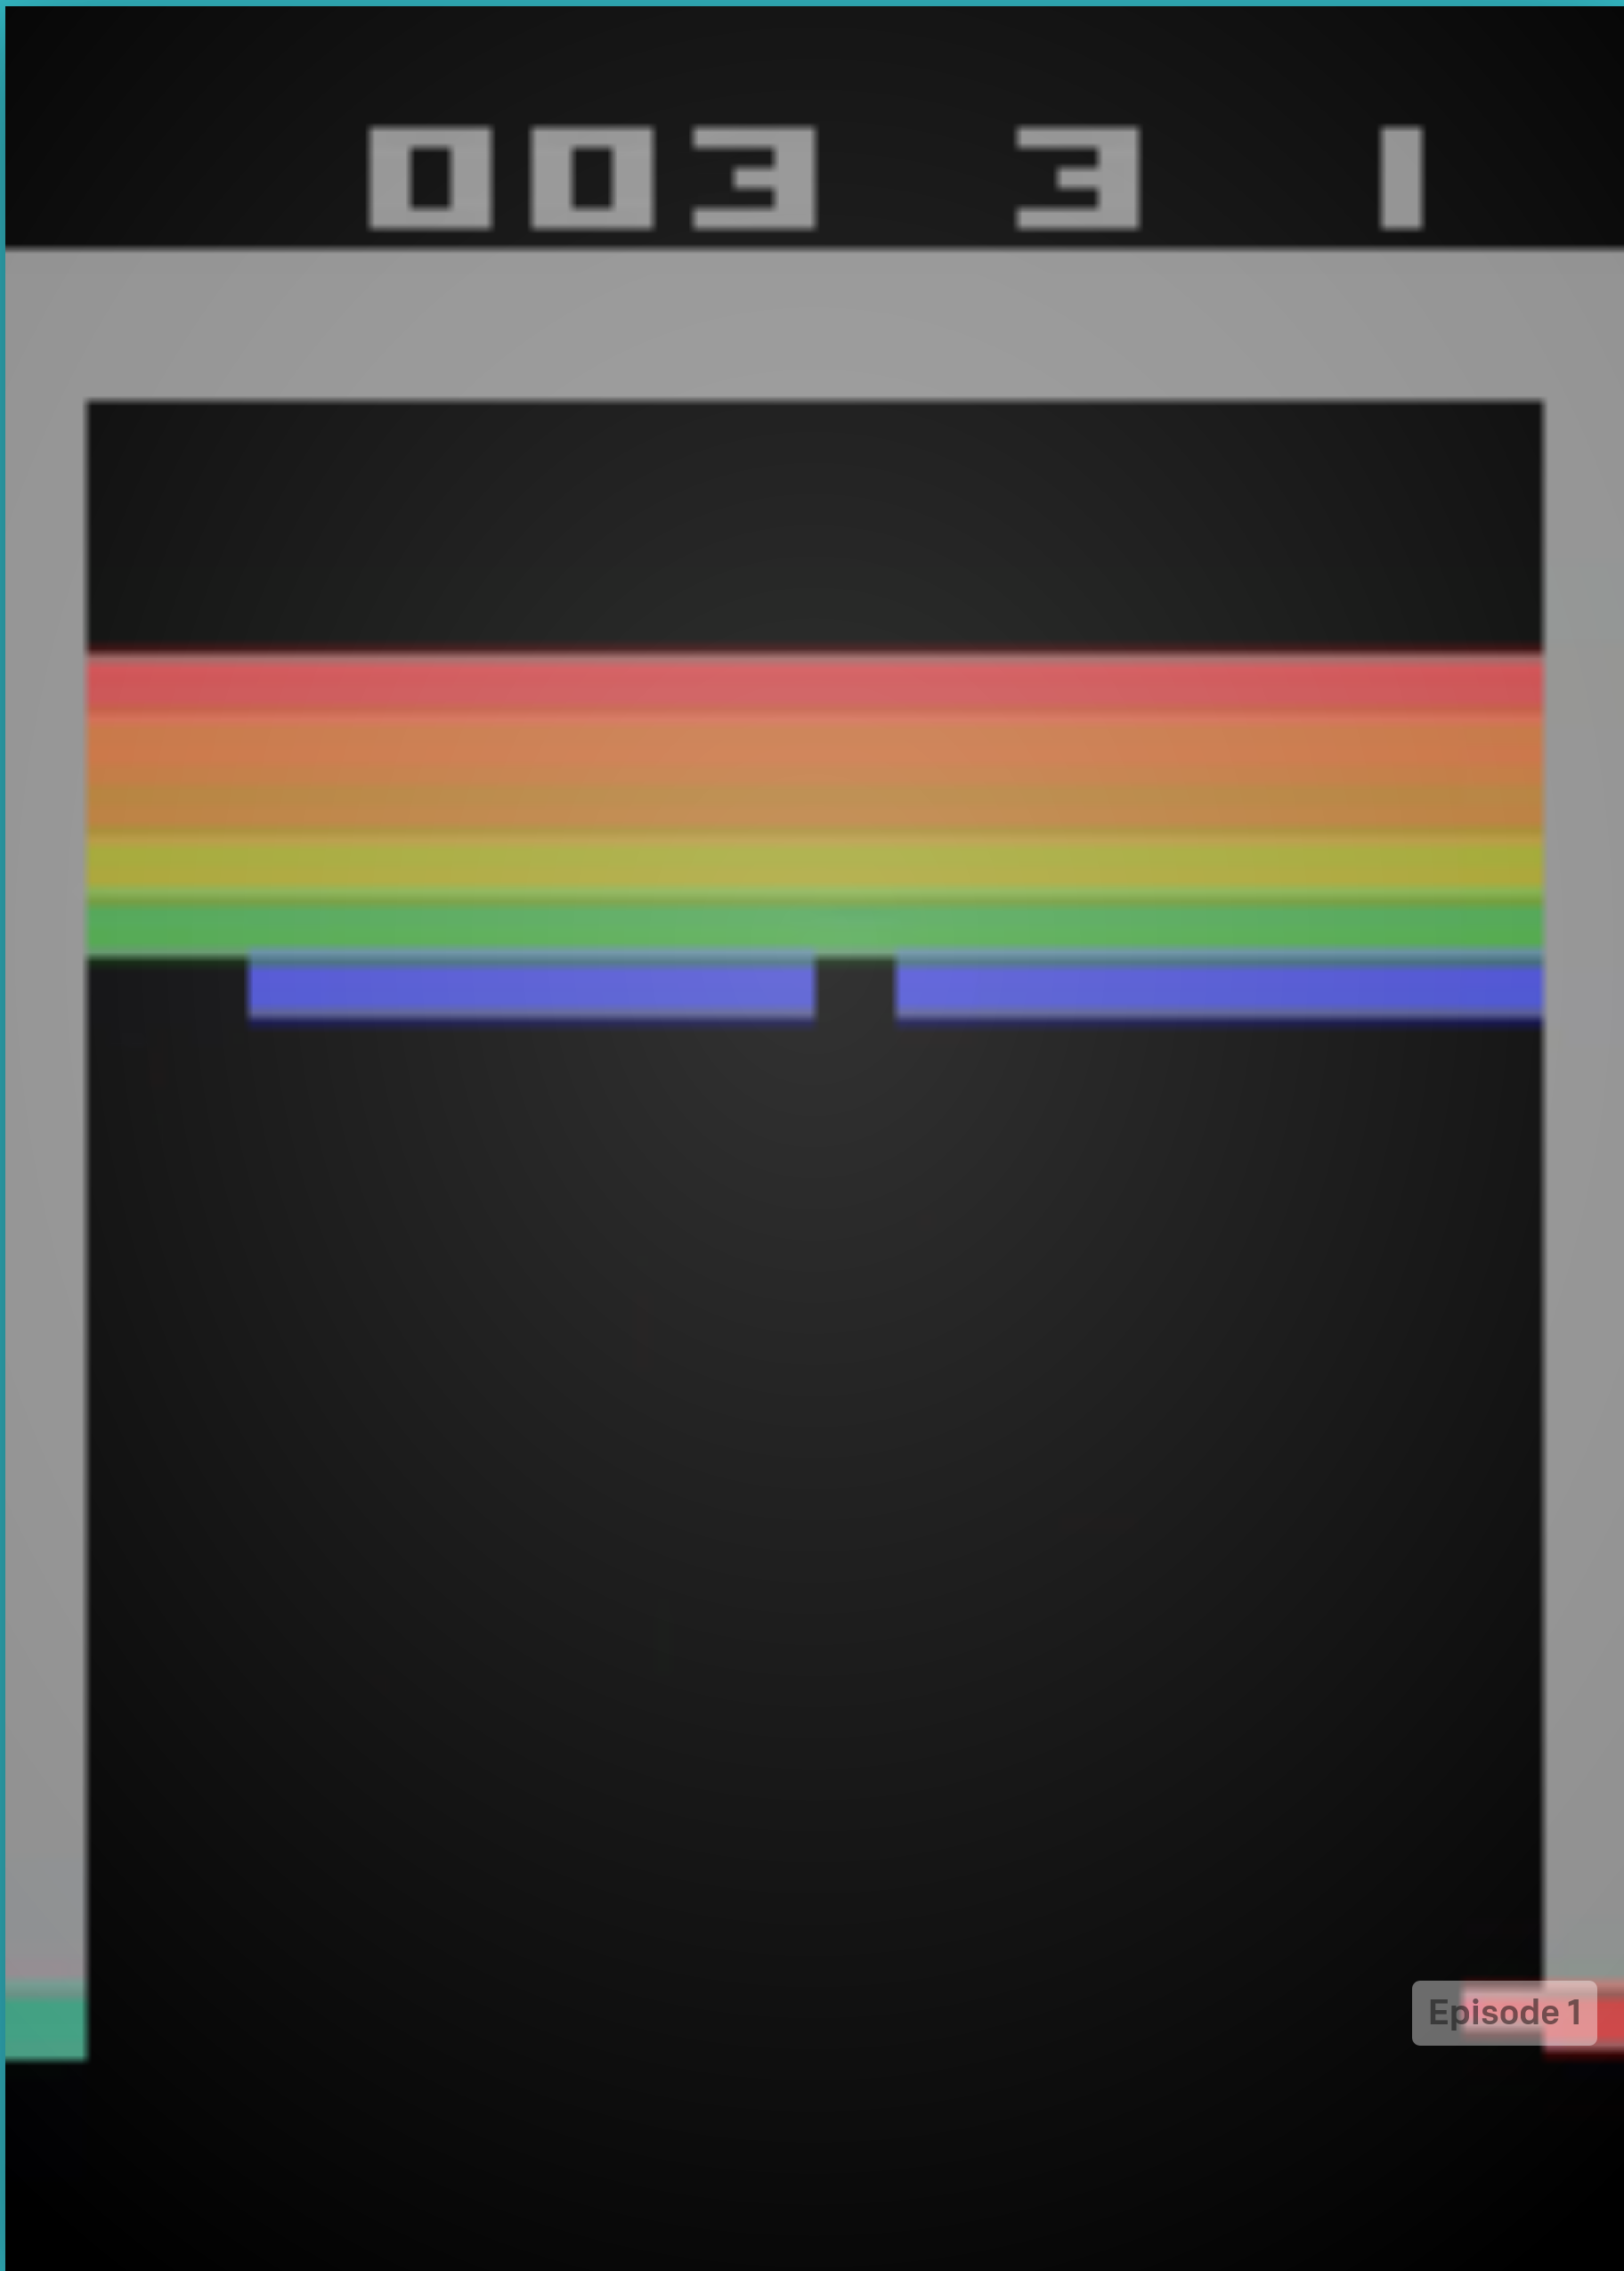
\includegraphics{breakout}
    \caption{The atari breakout envirement}
    \label{fig:breakout}
\end{marginfigure}

In this problem agent gets the same information as a human would, the pixels on the screen. Aditionally we give it the reward of the current timestep. Due to the computational complexity we do not want the agent to process the whole screen each timestep. We build our implementation on top of the \texttt{BreakoutDeterministic-v4} envirement provided by the \textit{openAI gym} project. This envirement returns the game state only once every 4 frames lowering the computational requirements.

\subsection{Implementation}
Initially we used a slightly adapted version of the mountain car DQN implementation described in \autoref{sec:mcar_impl}. The simple multilayer dense neural network was replaced with a convolutional neural network consisting of 2 layers both with kernal size 3 followed by two dense layers. The frames from the envirment where changed to greyscale and cropped to $80$ by $72$ pixels. This leaves the game envirement intact but removes the score at the top and ornamental edges, leaving an images as in \autoref{fig:breakout_postprocess} for the network.

This did not result in any learning by the agent. I tried multiple different networks before taking a look at related literature\cite{atari}. This lead to the conclusion that my agent was that my hyper paramaters where far from where they should be.

Taking the hyperparamaters from the famouse "Human-level control through deep reinforcement learning"\cite{DQN} we start changing the implementation. The mountain car agent is limited in the number of training sessions, this does not make sense for the breakout agent as we want to limit the number of steps not training sessions. From the perspective of a human traning there is no difference between losing a life and the game restarting however the agent was not even punished for losing a life. That was changed so losing a life is treated as losing the game during training.
Using only one frame as input to the network does not allow the agent to use the concept of direction or speed, essential to a human player. As in\cite{DQN} we feed the network a stack of the last 4 frames, as given to us by the envirement, for prediction and during training. 

\begin{marginfigure}
    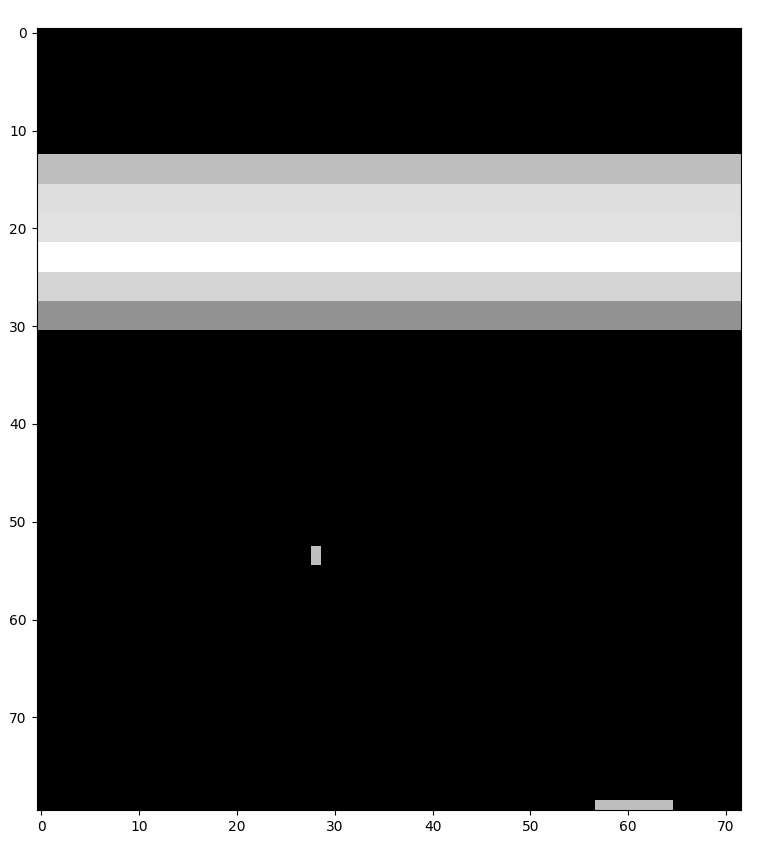
\includegraphics{network_input}
    \caption{A frame returned by the atari breakout envirement after postprocessing for our agent, converting to color and cropping out the unneeded edges}
    \label{fig:breakout_postprocess}
\end{marginfigure}

These changes give a number of implementation problems. We can not take any action for the first 3 timesteps as we can not make a stack of 4 frames to feed the agent. We have removed the training in sessions however we should not use frames from another training session. For example is the games has ended in frame $x$ we can not use the network until frame $x+4$. To enforce this we use the function \texttt{reset}. It resets the envirement and forwards the game 3 timesteps without taking any action. We use a new class \texttt{State} to keep track of the 4 frames. I provides a method \texttt{push} that takes as arguments an before and after state together with the action taken, score and if the game is over. It then forgets the oldest before and after state adding the new state to its internal stack.
This introduced a new problem, the stack of images drastically increased the memory requirements of the agent. Instead of single images the \texttt{event} inserted into the memory (see \autoref{sec:mcar_impl}) are a lot larger at $184$kB per state\footnote{frame before and after an action each $4$ images of $72\cdot80$ pixels, each pixel represented as a python floating point number of $8$ bytes giving a total of $184$kB per state. Multiplied by a million that becomes gigabytes}. If we want to have a replay buffer as in the literature\cite{DQN} of 1 million states the agent would need at least 184 gigabytes. I solved this in two steps. Instead of storing the pixels in the default floating point format they are stored as bytes. This does not lead to significant data loss as the envirment uses one byte per color per pixel, since we are using grayscale we can use a single byte per pixel. The \texttt{State} class is modified to cast pixels to bytes when a new frame is pushed. The \texttt{Predictor} class (see \autoref{sec:mcar_impl}) casts the pixels back to floats before feeding them to the convolutional neural network. By lowering the replay buffer size from one million to \nicefrac{1}{4} million. Later after the agent was run for 10 million steps the memory use was further reduced no longer saving 8 frames for each state but only two and recreating the full 8 frame states as they are sampled from the memory.
  I was able to train the agent for the full length of 10 million steps only once, I did a second run with 1 million steps. During the training for each game the score achieved, timesteps taken and final epsilon value where recorded. Achieving a heigher score is the primary goal for this agent. Taking more timesteps means the agent survives longer and has more opportunities to accidentily hit a block and score a poiont. For both training sessions I show the value of epsilon, the score and the timesteps per game vs training progress. For the score and timesteps per game we also plot a moving average created with a window size of 50. We expect score and timesteps per game to be highly correlated. 

\begin{figure}
    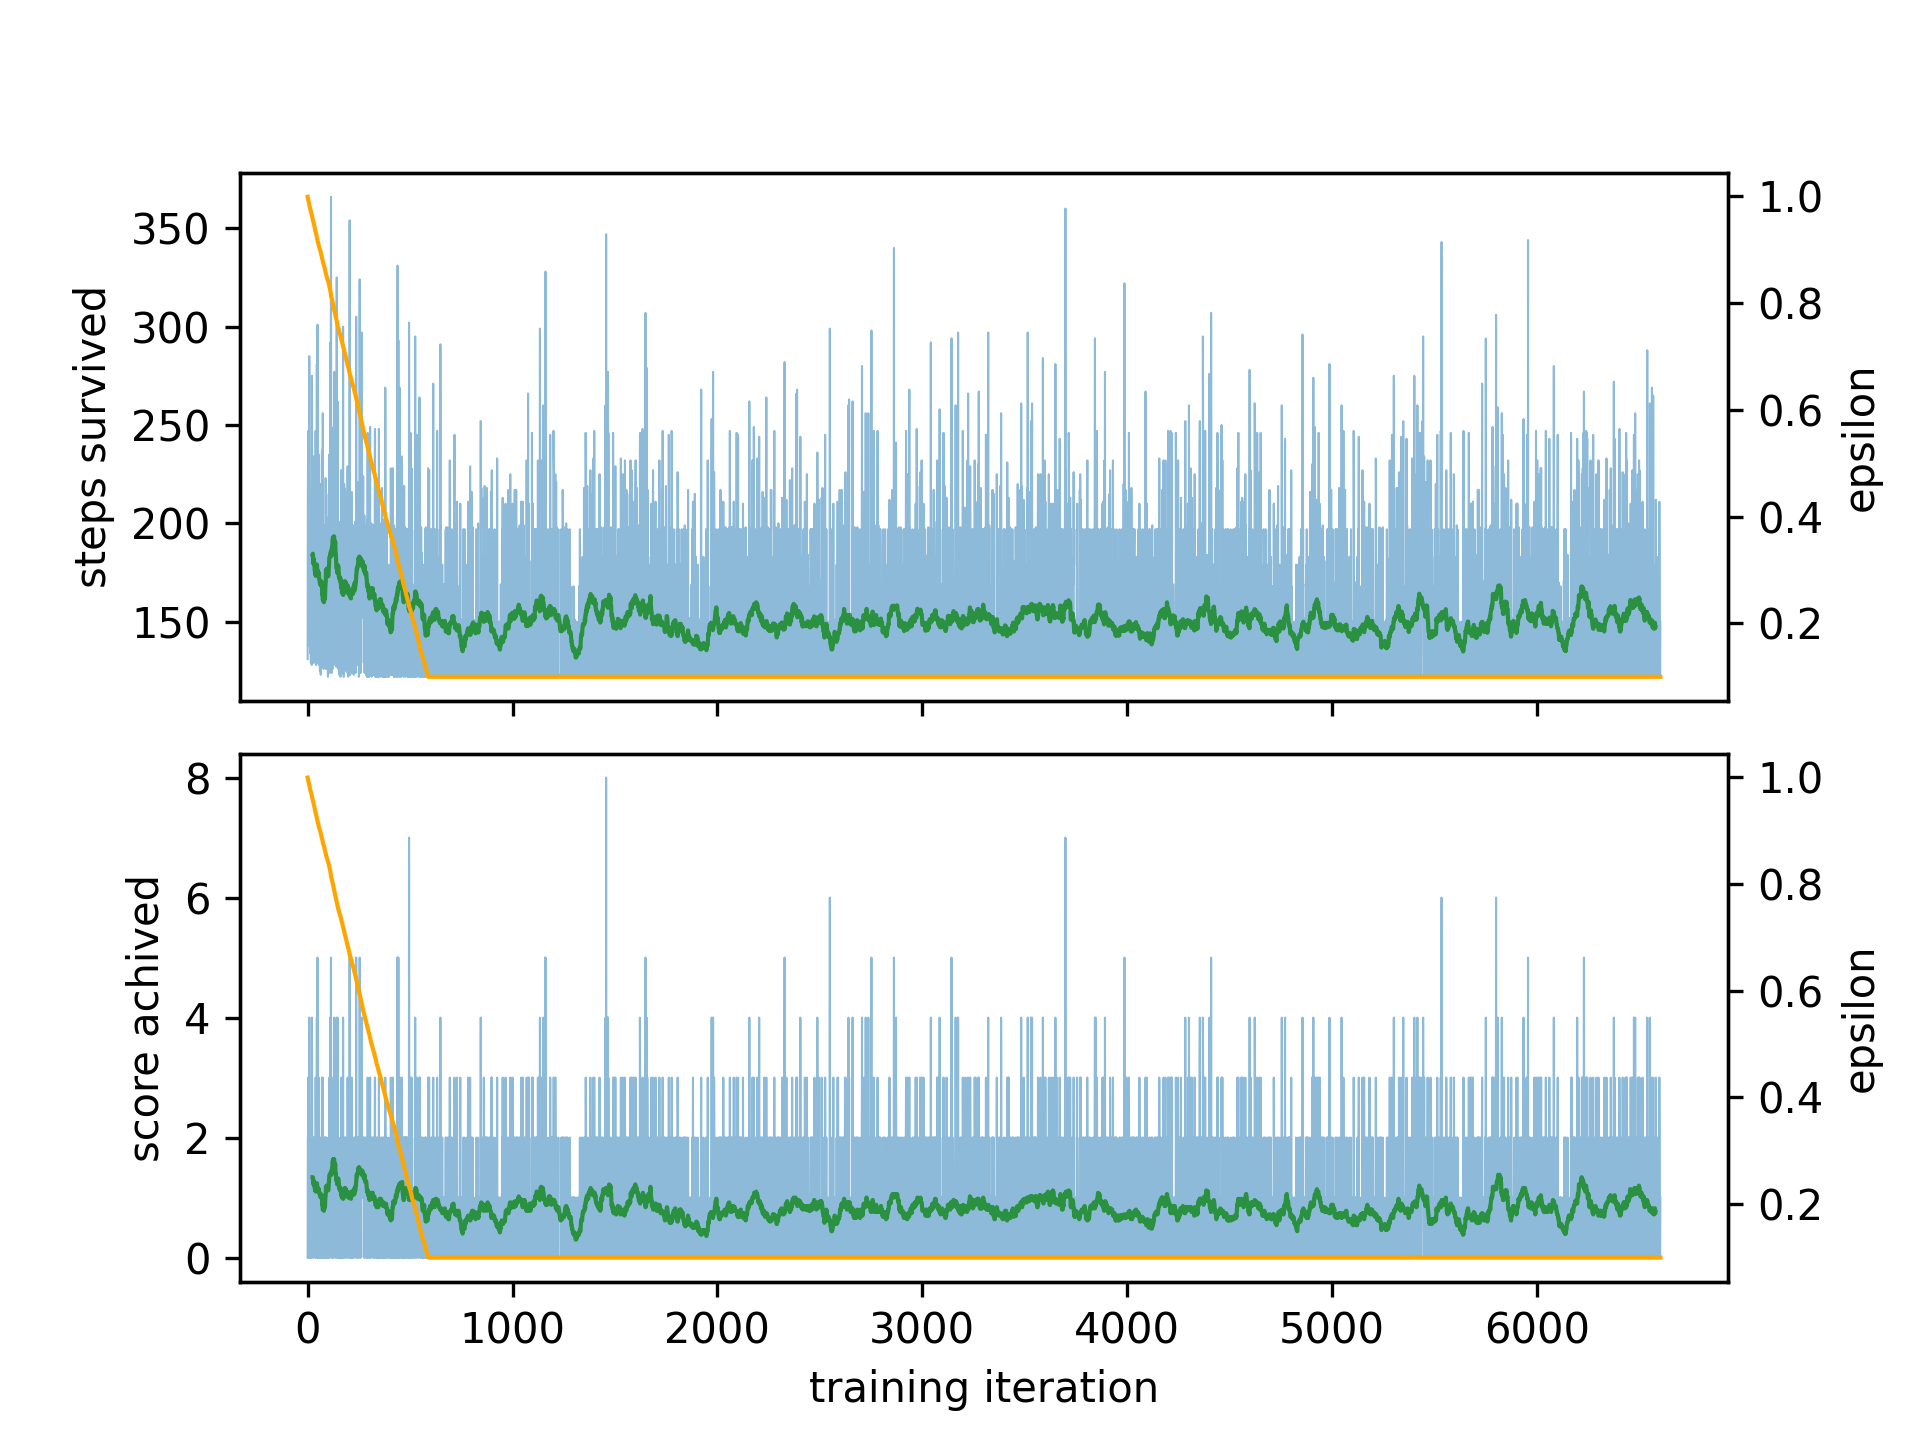
\includegraphics{breakout_1m}
    \caption{The performance of the agent when trained for 1 million steps. In orange the value of epsilon, in blue the steps per game for the top plot and score achived in the bottom plot. In green the moving average over the blue lines.}
    \label{fig:breakout_1m}
\end{figure}

In \autoref{fig:breakout_1m} we see how the agents performans during a training of 1 million steps. The behaviour of the agent is unstable it scores bad during the training not reaching howvering around a score of 1.2 which is the mean score for a random agent\cite{atari}. At around zero the agent seems take longer then later during training, I could not reproduce this thus attribute it to the randomness of the agent, especially as it mostly took random actions here due to the high epsilon value. 

When we train longer for 10 million steps we see a number of hopfull jumps before the agent jumps in performance around game $36000$, see \autoref{fig:breakout_10m}. 

\begin{figure}
    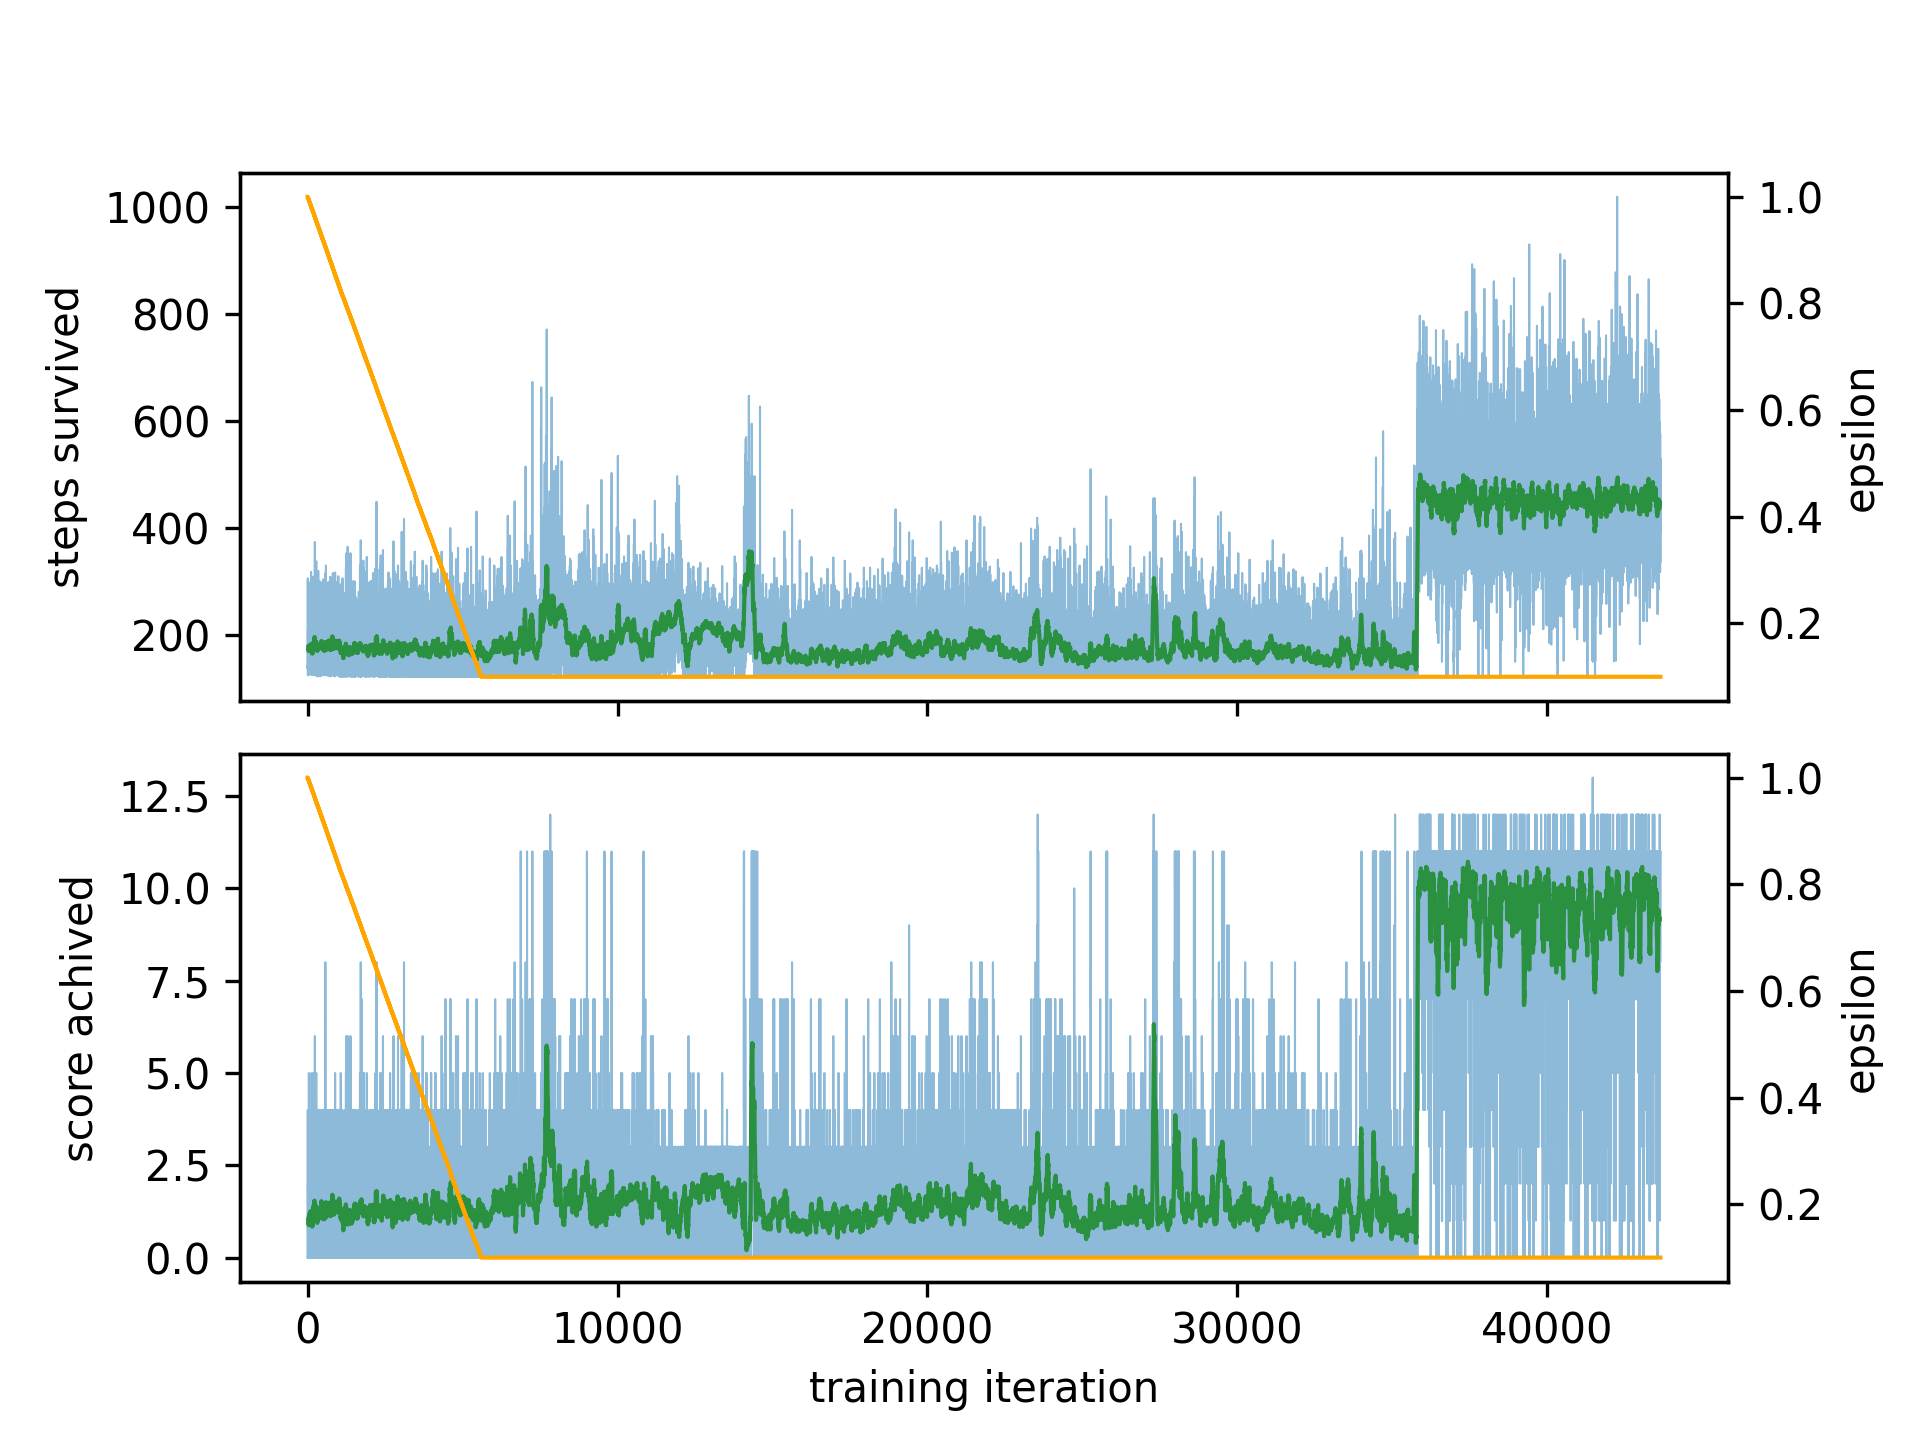
\includegraphics{breakout_10m}
    \caption{The performance of the agent when trained for 10 million steps. In orange the value of epsilon, in blue the steps per game for the top plot and score achived in the bottom plot. In green the moving average over the blue lines. For a closer look at the jump in performance around game $36000$ see \autoref{fig:breakout_10m_zoomed}}
    \label{fig:breakout_10m}
\end{figure}

From the moving average (green) we clearly see the agent had two early peaks where it seemd to grasp the game for a short while before collapsing again. Looking closer at the later jump (\autoref{fig:breakout_10m_zoomed}) note the improvement is quite a sudden, within 20 games the agent has grasped the basics of the game and is far outperforming its previous self only failing incidentilly. However we also see that save for one a single peak the agent never exceeds a score of 12.

\begin{figure}
    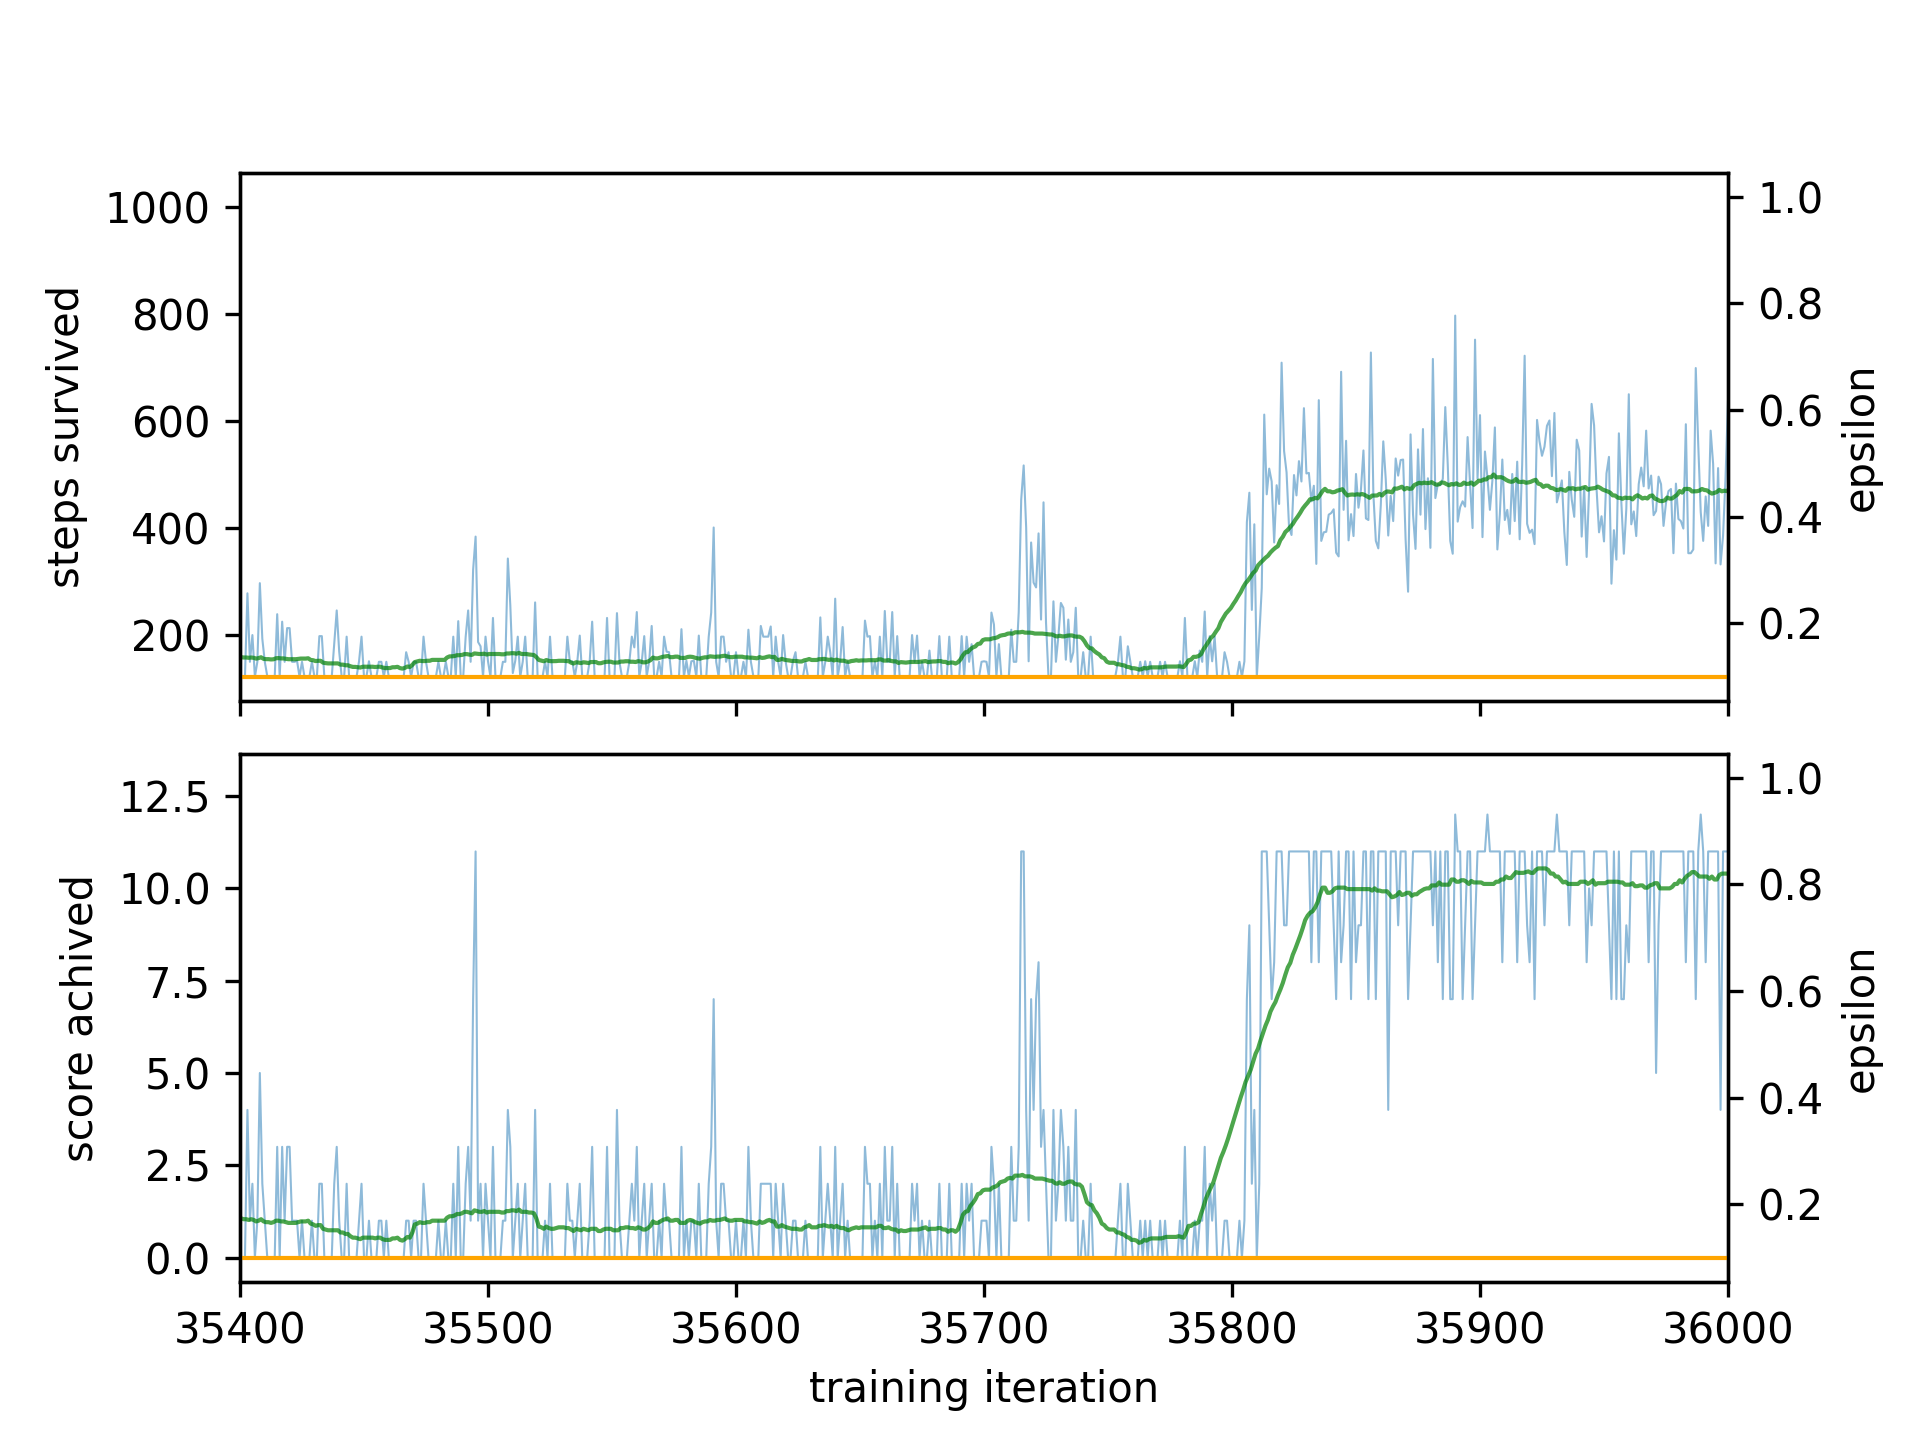
\includegraphics{breakout_10m_zoomed}
    \caption{The performance of the agent when it jumps up in performance at around game $36000$. In orange the value of epsilon, in blue the steps per game for the top plot and score achived in the bottom plot. In green the moving average over the blue lines.}
    \label{fig:breakout_10m_zoomed}
\end{figure}

  \chapter{Breakout}
  \label{sec:breakout}
Here the agent needs to master the atari game breakout, see \autoref{fig:breakout}. The agent controls a small bar at the bottem of the screen with possible actions: move left, move right or stay. A ball moves with constant speed through the envirement. If the agent positions the small bar such that the ball hits the bar the ball inverts its vertical velocity bouncing upwards. Whenever the ball hits the bottem of the screen it disappears, the agent loses a life (it starts with 5) and a new ball is introduced with a random direction downwards. When the ball hits the left and right side of the screen the horizontal velocity is inverted making it bounce of the walls. Somewhat below the top of the screen is a stack of rows of blocks. Whenever the ball hits one of the blocks: the block disappears, the ball inverts its vertical velocity and the agent is rewarded with score one for the current timestep. If the ball hits the top of the screen its vertical velocity is inverted, bouncing it off the top. 

\begin{marginfigure}
    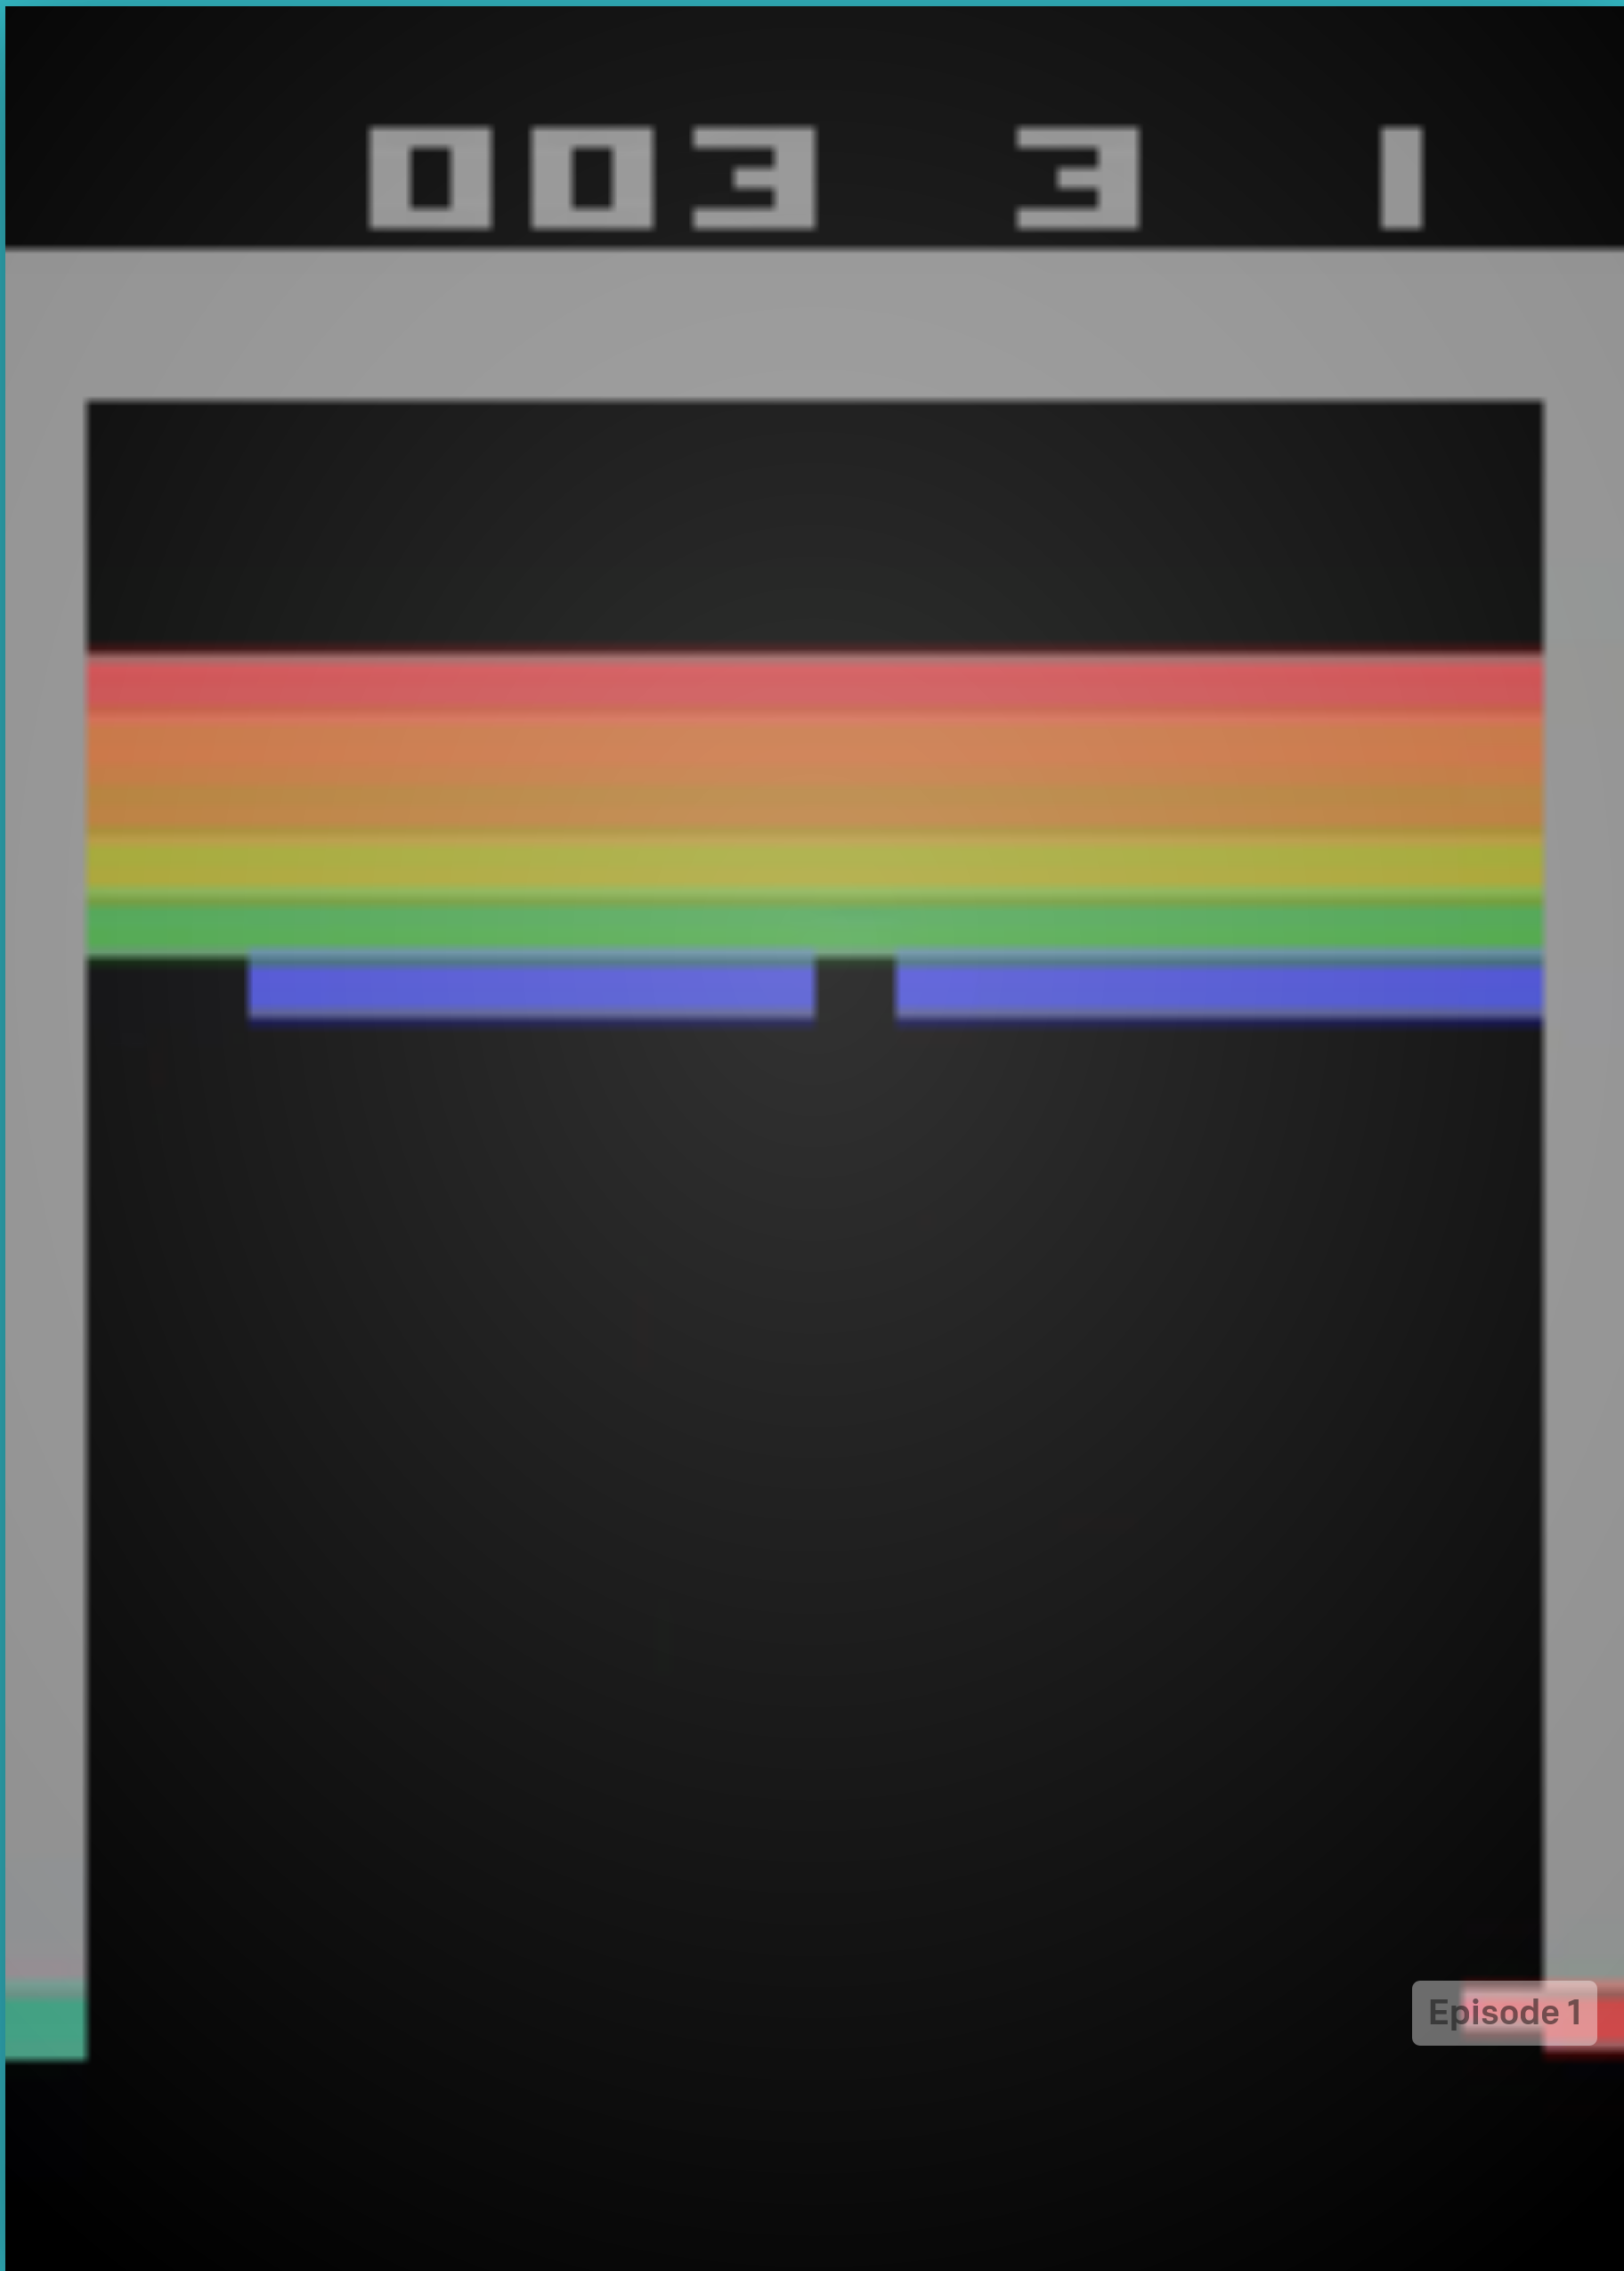
\includegraphics{breakout}
    \caption{The atari breakout envirement}
    \label{fig:breakout}
\end{marginfigure}

In this problem agent gets the same information as a human would, the pixels on the screen. Aditionally we give it the reward of the current timestep. Due to the computational complexity we do not want the agent to process the whole screen each timestep. We build our implementation on top of the \texttt{BreakoutDeterministic-v4} envirement provided by the \textit{openAI gym} project. This envirement returns the game state only once every 4 frames lowering the computational requirements.

\subsection{Implementation}
Initially we used a slightly adapted version of the mountain car DQN implementation described in \autoref{sec:mcar_impl}. The simple multilayer dense neural network was replaced with a convolutional neural network consisting of 2 layers both with kernal size 3 followed by two dense layers. The frames from the envirment where changed to greyscale and cropped to $80$ by $72$ pixels. This leaves the game envirement intact but removes the score at the top and ornamental edges, leaving an images as in \autoref{fig:breakout_postprocess} for the network.

This did not result in any learning by the agent. I tried multiple different networks before taking a look at related literature\cite{atari}. This lead to the conclusion that my agent was that my hyper paramaters where far from where they should be.

Taking the hyperparamaters from the famouse "Human-level control through deep reinforcement learning"\cite{DQN} we start changing the implementation. The mountain car agent is limited in the number of training sessions, this does not make sense for the breakout agent as we want to limit the number of steps not training sessions. From the perspective of a human traning there is no difference between losing a life and the game restarting however the agent was not even punished for losing a life. That was changed so losing a life is treated as losing the game during training.
Using only one frame as input to the network does not allow the agent to use the concept of direction or speed, essential to a human player. As in\cite{DQN} we feed the network a stack of the last 4 frames, as given to us by the envirement, for prediction and during training. 

\begin{marginfigure}
    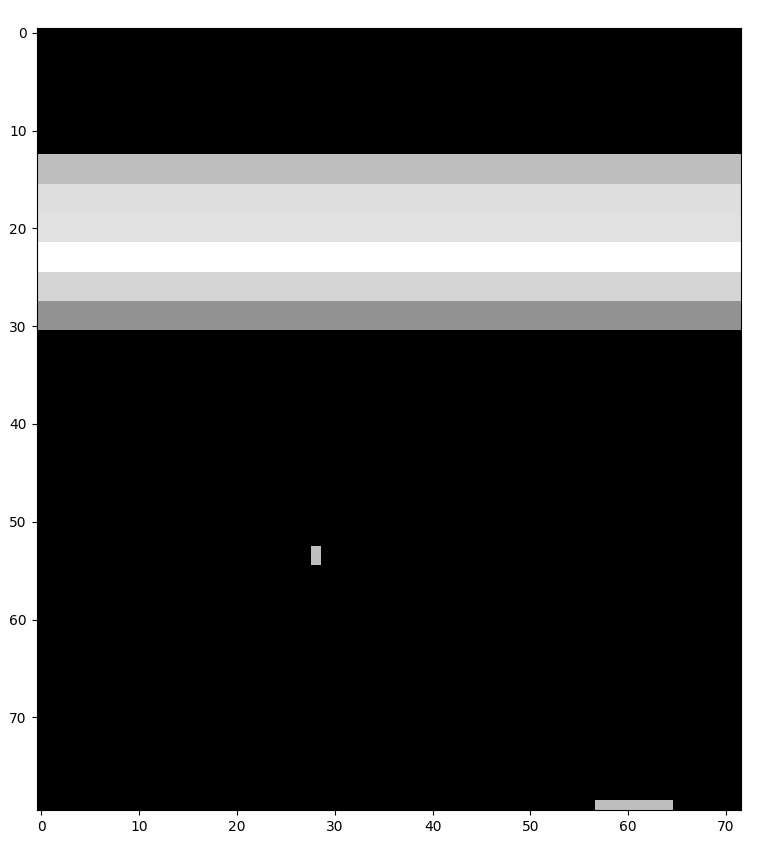
\includegraphics{network_input}
    \caption{A frame returned by the atari breakout envirement after postprocessing for our agent, converting to color and cropping out the unneeded edges}
    \label{fig:breakout_postprocess}
\end{marginfigure}

These changes give a number of implementation problems. We can not take any action for the first 3 timesteps as we can not make a stack of 4 frames to feed the agent. We have removed the training in sessions however we should not use frames from another training session. For example is the games has ended in frame $x$ we can not use the network until frame $x+4$. To enforce this we use the function \texttt{reset}. It resets the envirement and forwards the game 3 timesteps without taking any action. We use a new class \texttt{State} to keep track of the 4 frames. I provides a method \texttt{push} that takes as arguments an before and after state together with the action taken, score and if the game is over. It then forgets the oldest before and after state adding the new state to its internal stack.
This introduced a new problem, the stack of images drastically increased the memory requirements of the agent. Instead of single images the \texttt{event} inserted into the memory (see \autoref{sec:mcar_impl}) are a lot larger at $184$kB per state\footnote{frame before and after an action each $4$ images of $72\cdot80$ pixels, each pixel represented as a python floating point number of $8$ bytes giving a total of $184$kB per state. Multiplied by a million that becomes gigabytes}. If we want to have a replay buffer as in the literature\cite{DQN} of 1 million states the agent would need at least 184 gigabytes. I solved this in two steps. Instead of storing the pixels in the default floating point format they are stored as bytes. This does not lead to significant data loss as the envirment uses one byte per color per pixel, since we are using grayscale we can use a single byte per pixel. The \texttt{State} class is modified to cast pixels to bytes when a new frame is pushed. The \texttt{Predictor} class (see \autoref{sec:mcar_impl}) casts the pixels back to floats before feeding them to the convolutional neural network. By lowering the replay buffer size from one million to \nicefrac{1}{4} million. Later after the agent was run for 10 million steps the memory use was further reduced no longer saving 8 frames for each state but only two and recreating the full 8 frame states as they are sampled from the memory.
  I was able to train the agent for the full length of 10 million steps only once, I did a second run with 1 million steps. During the training for each game the score achieved, timesteps taken and final epsilon value where recorded. Achieving a heigher score is the primary goal for this agent. Taking more timesteps means the agent survives longer and has more opportunities to accidentily hit a block and score a poiont. For both training sessions I show the value of epsilon, the score and the timesteps per game vs training progress. For the score and timesteps per game we also plot a moving average created with a window size of 50. We expect score and timesteps per game to be highly correlated. 

\begin{figure}
    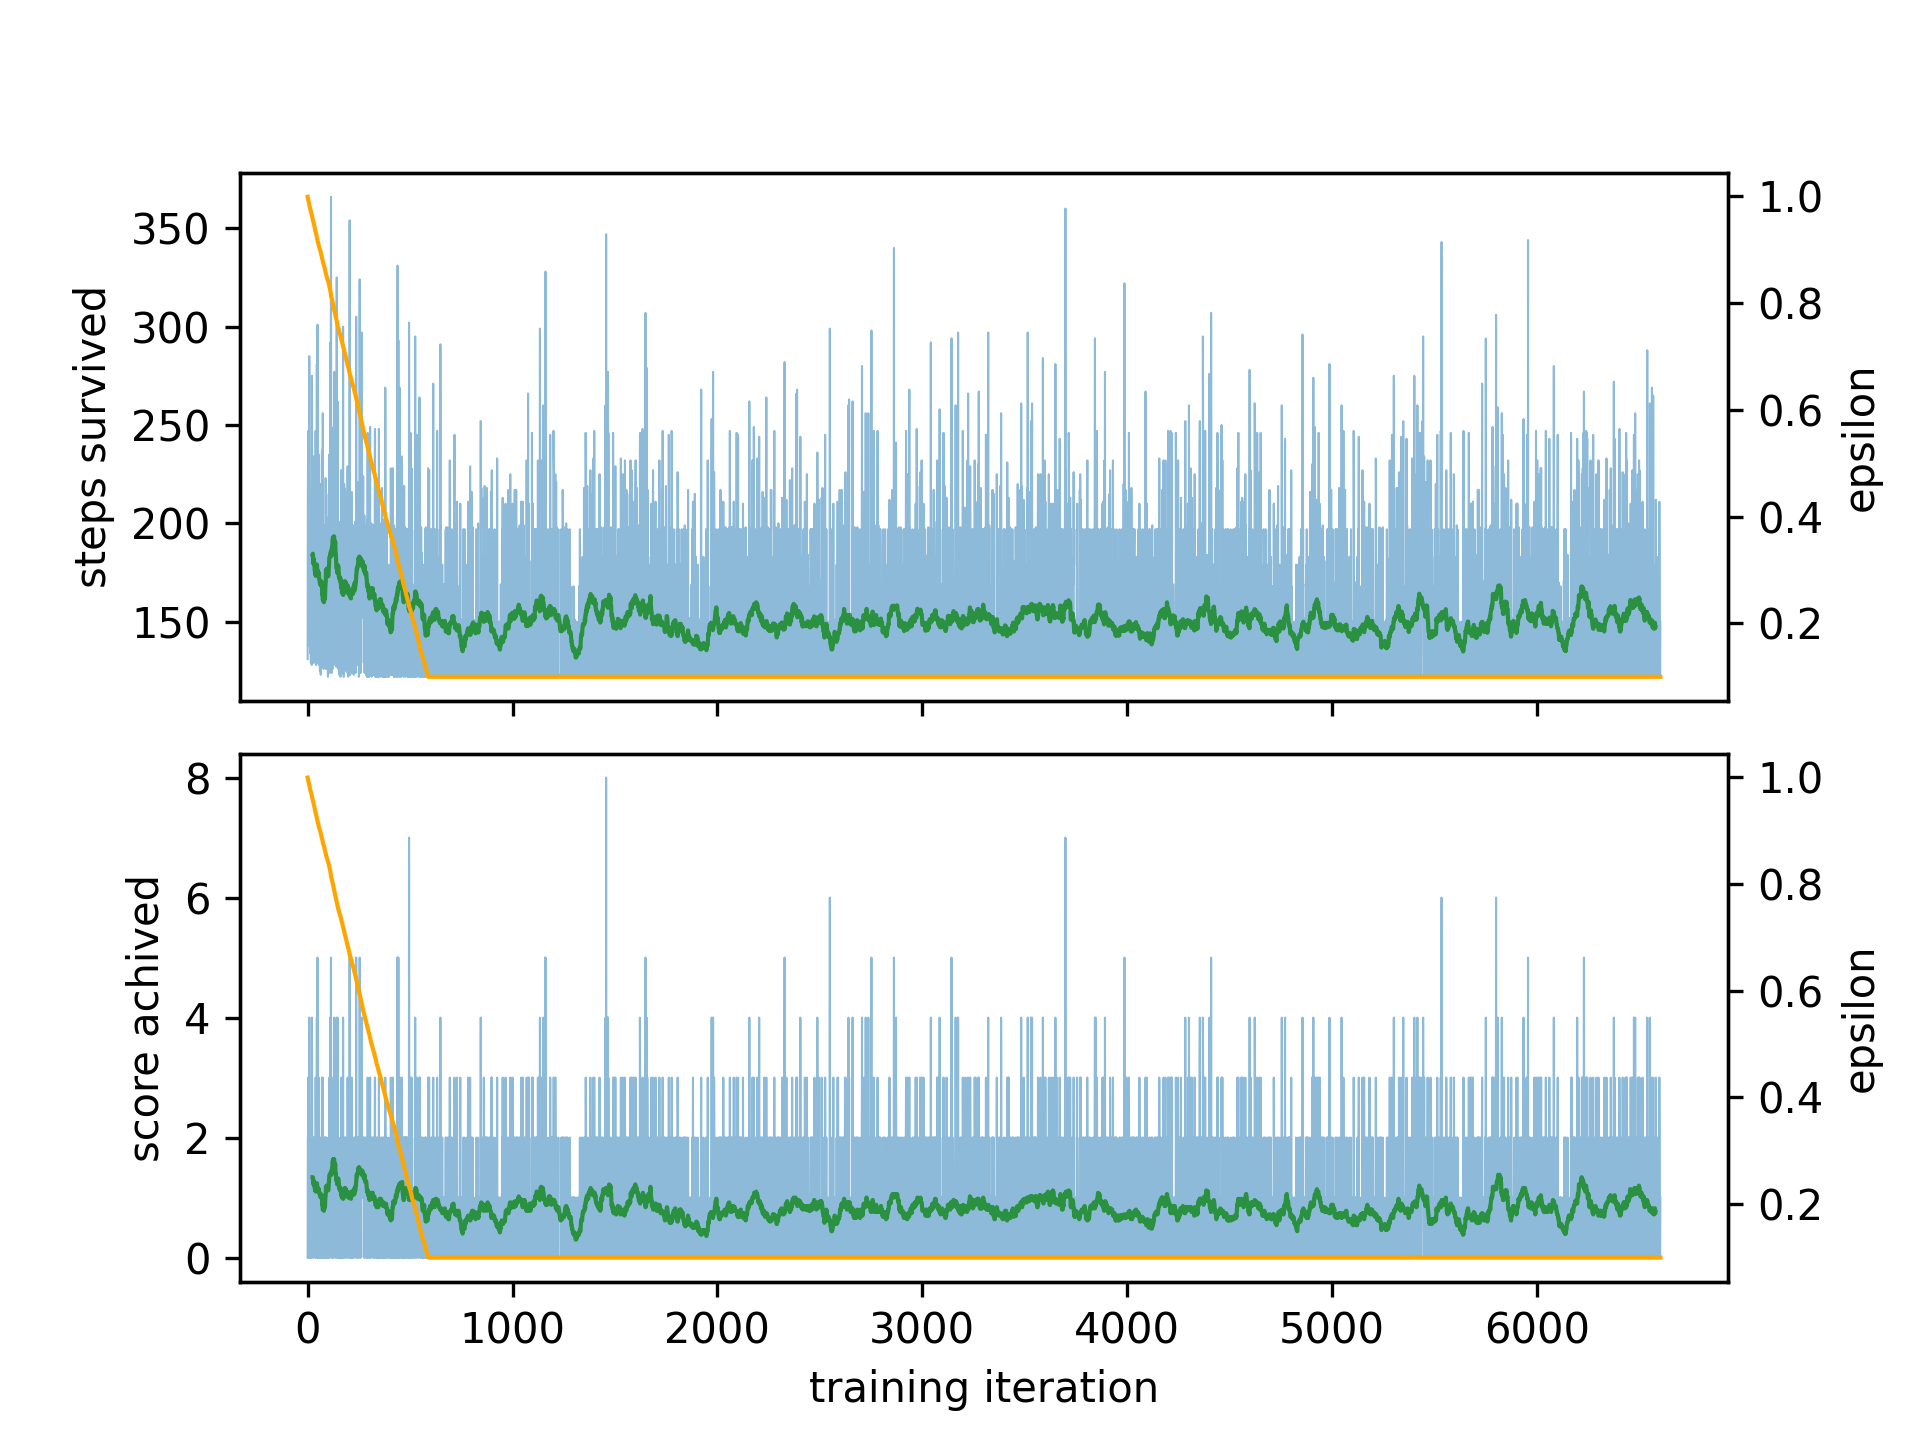
\includegraphics{breakout_1m}
    \caption{The performance of the agent when trained for 1 million steps. In orange the value of epsilon, in blue the steps per game for the top plot and score achived in the bottom plot. In green the moving average over the blue lines.}
    \label{fig:breakout_1m}
\end{figure}

In \autoref{fig:breakout_1m} we see how the agents performans during a training of 1 million steps. The behaviour of the agent is unstable it scores bad during the training not reaching howvering around a score of 1.2 which is the mean score for a random agent\cite{atari}. At around zero the agent seems take longer then later during training, I could not reproduce this thus attribute it to the randomness of the agent, especially as it mostly took random actions here due to the high epsilon value. 

When we train longer for 10 million steps we see a number of hopfull jumps before the agent jumps in performance around game $36000$, see \autoref{fig:breakout_10m}. 

\begin{figure}
    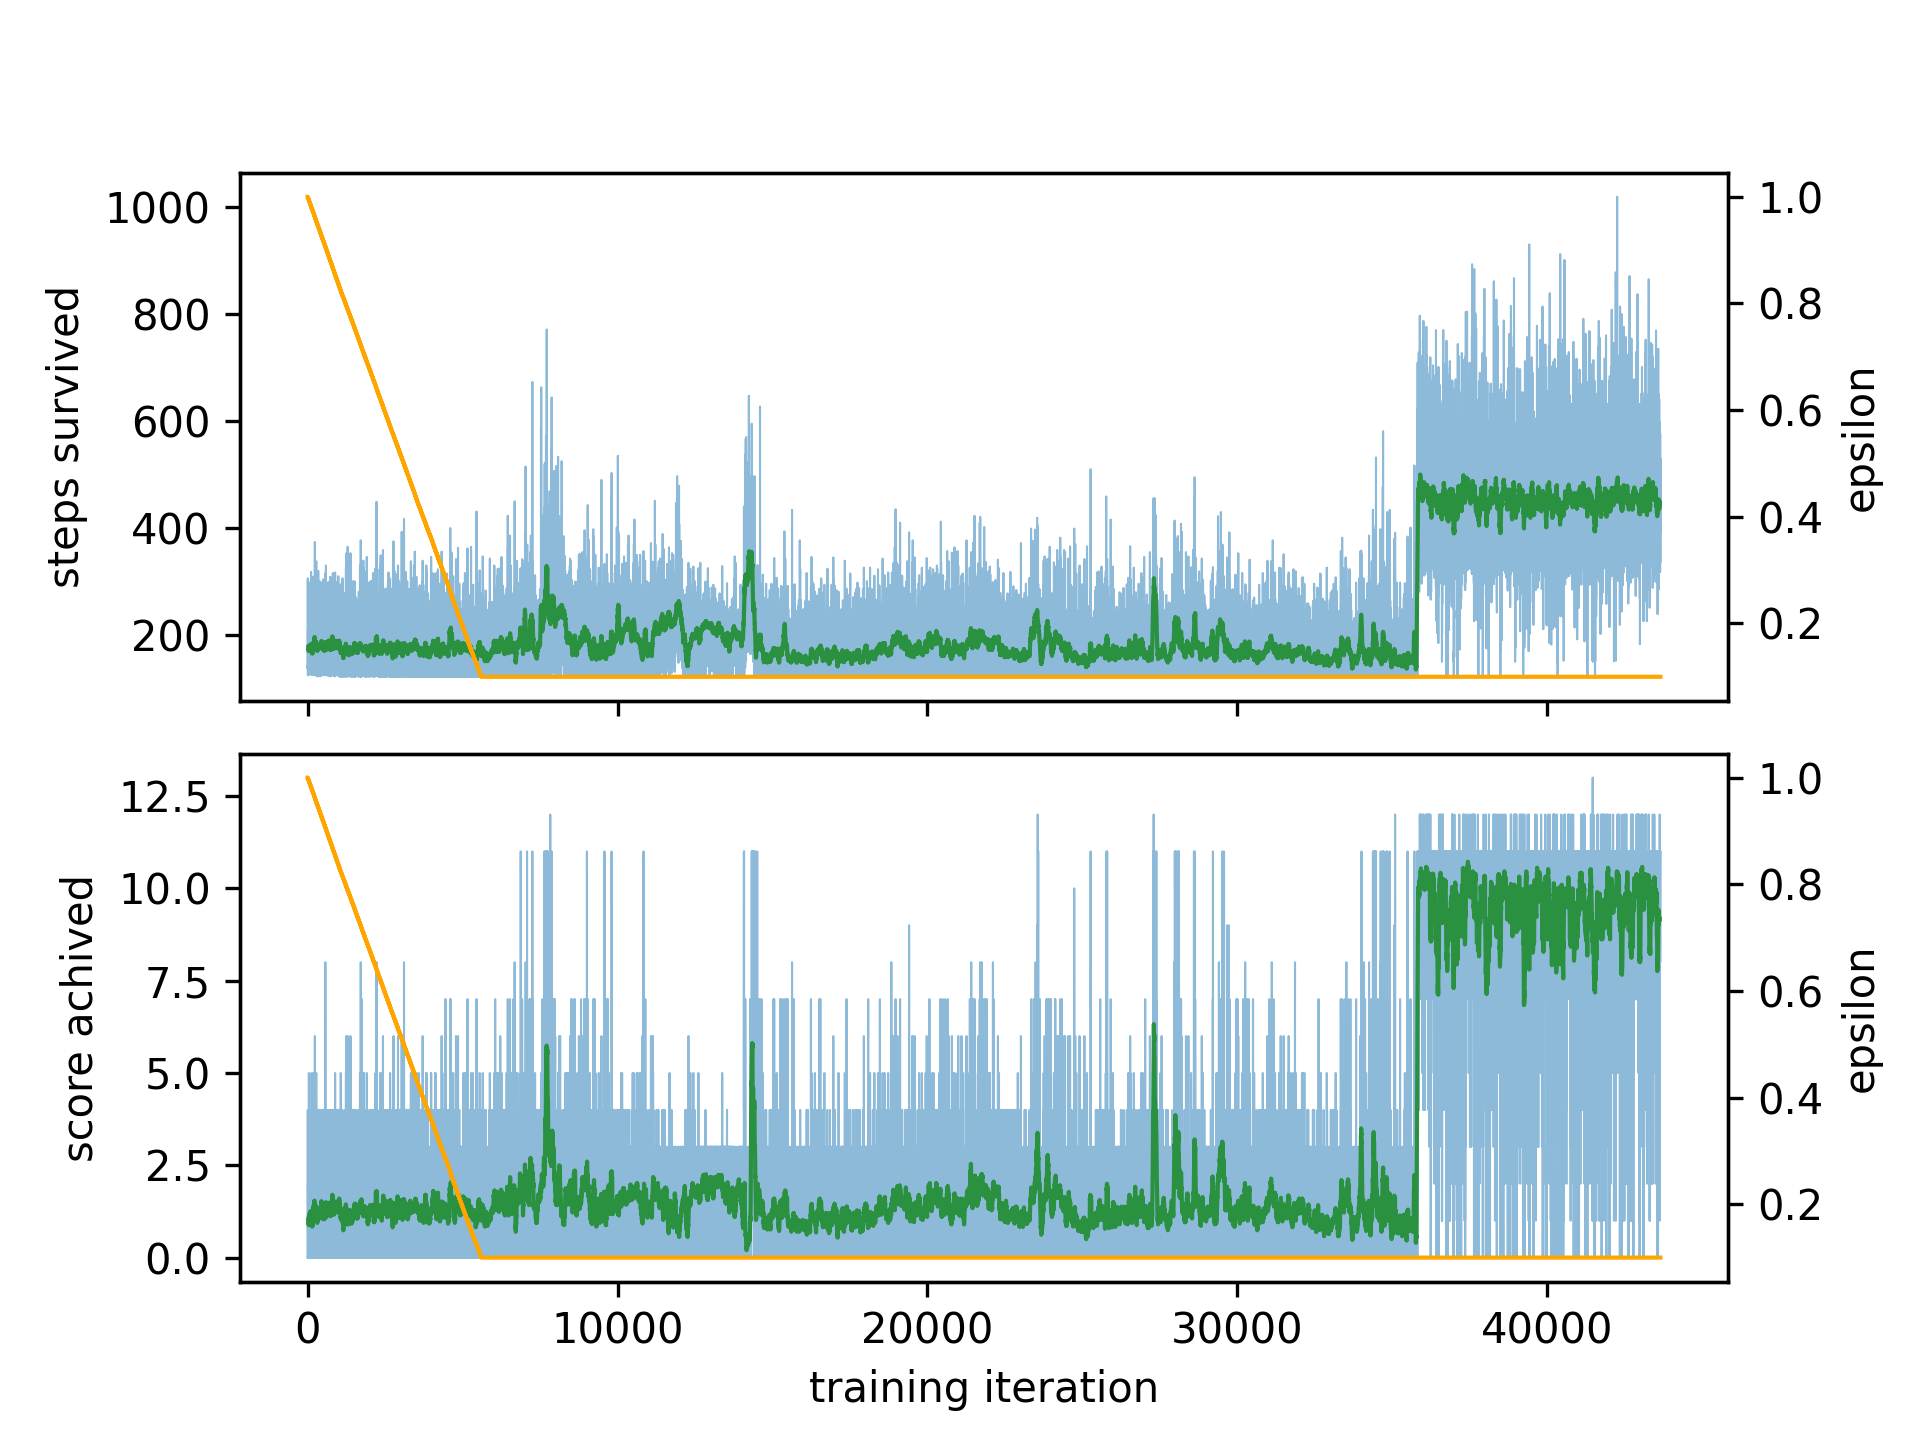
\includegraphics{breakout_10m}
    \caption{The performance of the agent when trained for 10 million steps. In orange the value of epsilon, in blue the steps per game for the top plot and score achived in the bottom plot. In green the moving average over the blue lines. For a closer look at the jump in performance around game $36000$ see \autoref{fig:breakout_10m_zoomed}}
    \label{fig:breakout_10m}
\end{figure}

From the moving average (green) we clearly see the agent had two early peaks where it seemd to grasp the game for a short while before collapsing again. Looking closer at the later jump (\autoref{fig:breakout_10m_zoomed}) note the improvement is quite a sudden, within 20 games the agent has grasped the basics of the game and is far outperforming its previous self only failing incidentilly. However we also see that save for one a single peak the agent never exceeds a score of 12.

\begin{figure}
    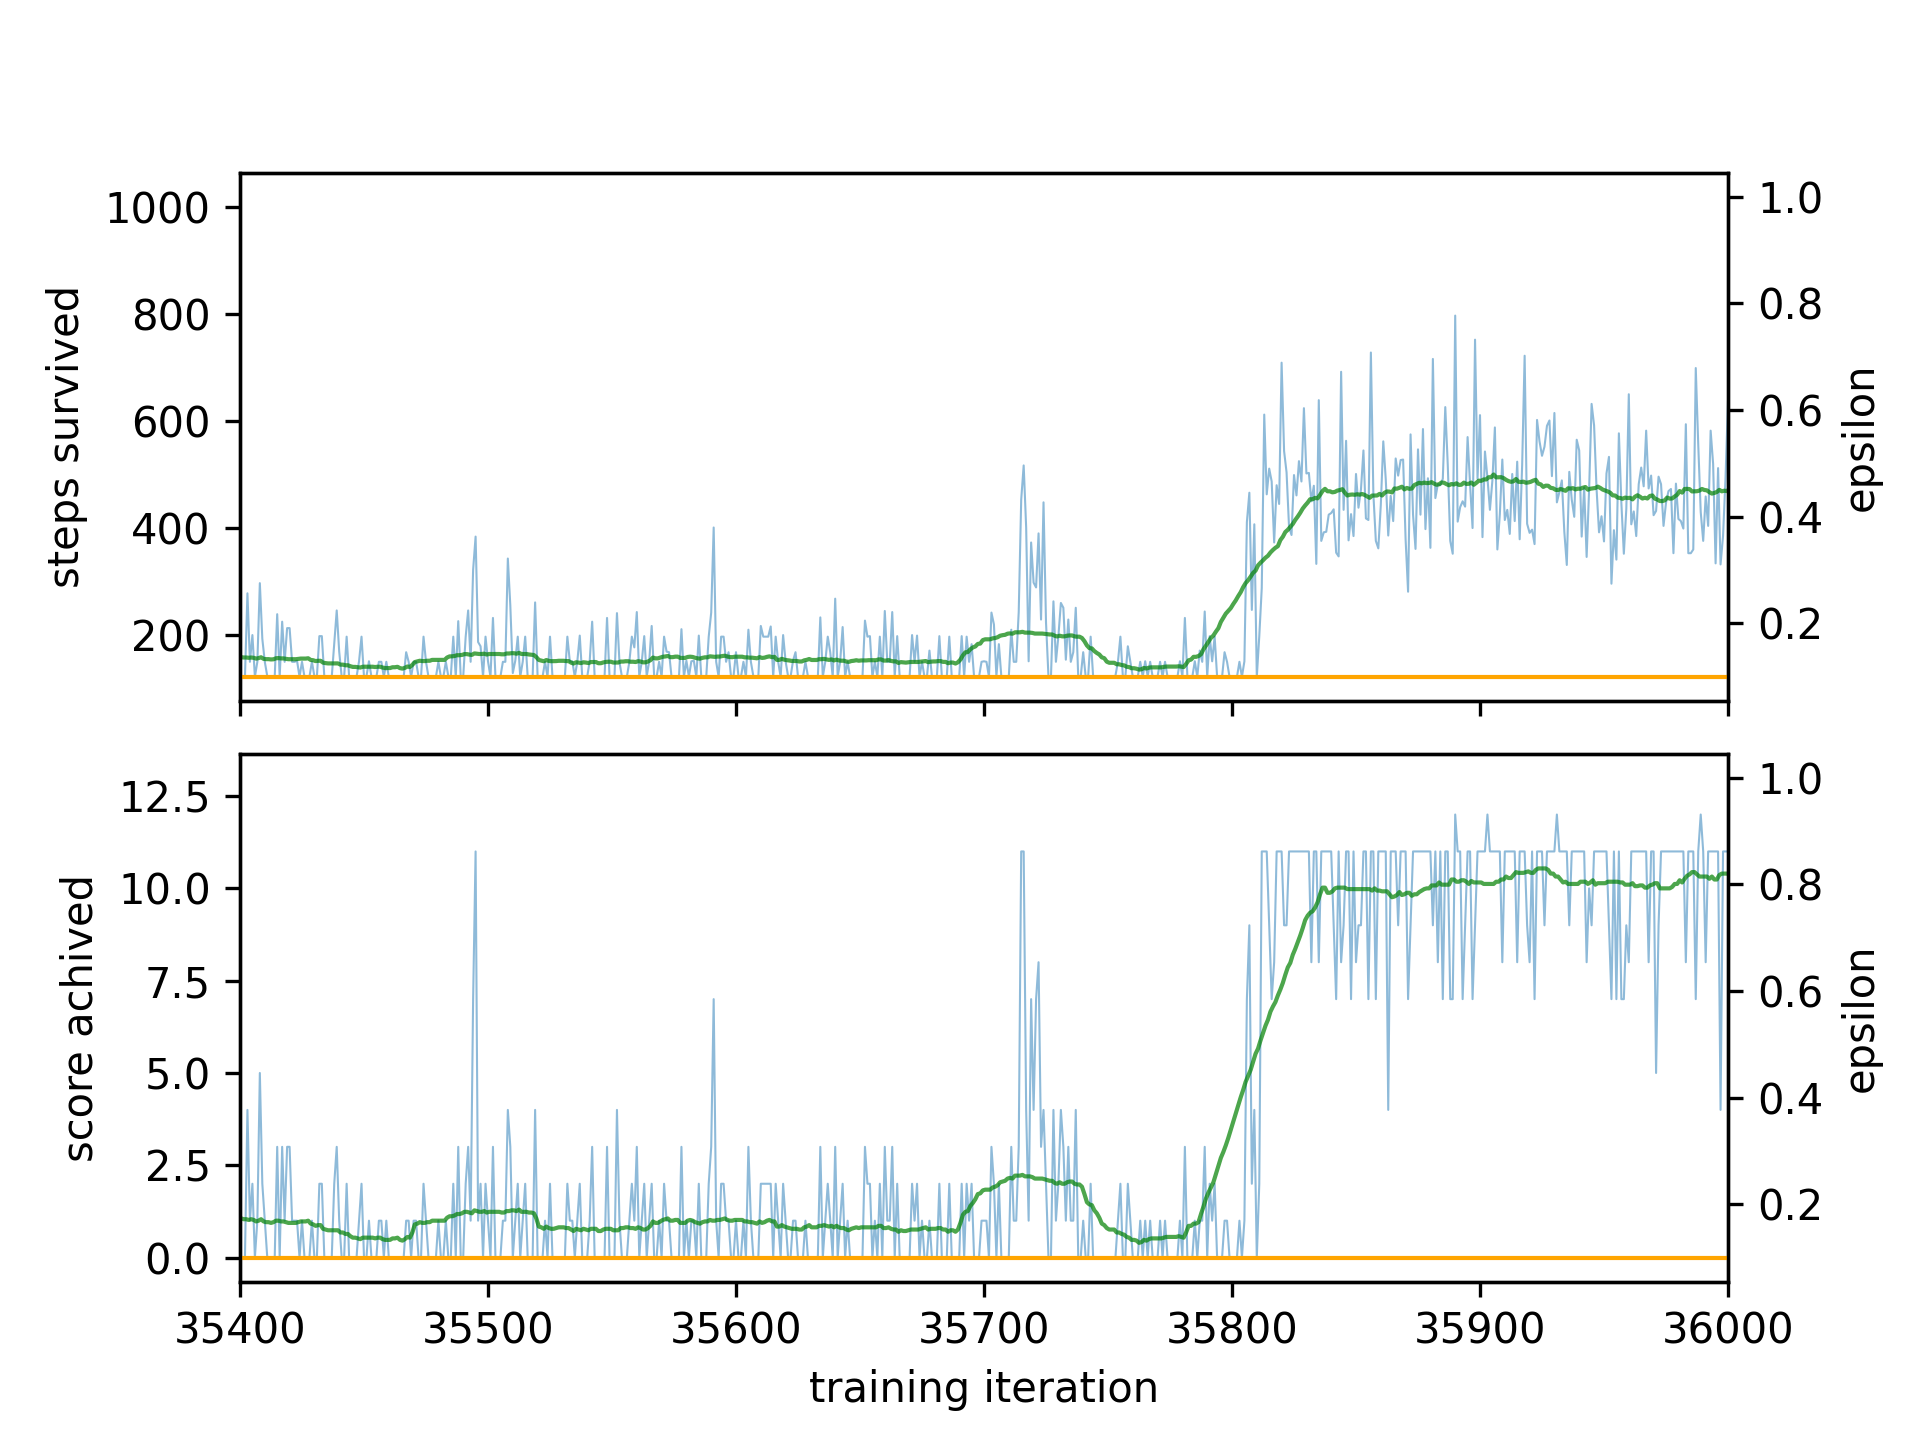
\includegraphics{breakout_10m_zoomed}
    \caption{The performance of the agent when it jumps up in performance at around game $36000$. In orange the value of epsilon, in blue the steps per game for the top plot and score achived in the bottom plot. In green the moving average over the blue lines.}
    \label{fig:breakout_10m_zoomed}
\end{figure}

  \chapter{Conclusion}
  

//future work:
- reset light on live lost
- State only needs the after states
- prediction should be done on the stack of after states

% This ensures that the subsequent sections are being included as root
% items in the bookmark structure of your PDF reader.
\bookmarksetup{startatroot}
\backmatter

  \begingroup
    \let\clearpage\relax
    \glsaddall
    \printglossary[type=\acronymtype]
    \newpage
    \printglossary
  \endgroup

  \printindex
  \printbibliography

\end{document}